
\documentclass[10pt]{article}

\usepackage{epsfig}
\usepackage{verbatim}
\usepackage{underscore}
\usepackage{hyperref}
\hypersetup{
    colorlinks=true,
    urlcolor=blue,
    linkcolor=black,
}

\parskip=.080in
\setlength{\evensidemargin}{-0.2in}
\setlength{\oddsidemargin}{-0.2in}
\setlength{\parindent}{0.0in}
\setlength{\textwidth}{6.9in}
\setlength{\topmargin}{-0.5in}
\setlength{\textheight}{10.0in}
\setlength{\headheight}{0in}
\setlength{\headsep}{0in}
\setlength{\topsep}{0in}
\setlength{\itemsep}{0in}
\renewcommand{\baselinestretch}{1.1}
\pagestyle{empty}

%%%%%%%%%%%%%%%%%%%%%%%%%%%%%%%%%%%%%%%%%%%%%%%%%%%%%%%%%%%%%%%%%%%%
%%%%%%%%%%%%%%%%%%%%%%%%%%%%%%%%%%%%%%%%%%%%%%%%%%%%%%%%%%%%%%%%%%%%
%%%%%%%%%%%%%%%%%%%%%%%%%%%%%%%%%%%%%%%%%%%%%%%%%%%%%%%%%%%%%%%%%%%%

\begin{document}

\Large
{\bf Project 1 Technical Specification}\\
{\bf \noindent CS621: Network Programming -- Spring 2019}\\
\noindent \emph{Updated: Feb 5th, 2019}\\

\normalsize
\setcounter{secnumdepth}{0}
\section{Project Outcomes}
\begin{enumerate}
    \item Enable network compression for point-to-point links in ns-3.
    \item Implement the network application that detects the presence of network compression by end-hosts.
    \item Verify and validate your simulated compression link and compression detection application.
\end{enumerate}

\section{Overview}
For this project you will implement a network level compression link. You will then implement a network application to detect whether network compression is present to validate your simulated compression link. It is inspired by the work, \href{https://lasr.cs.ucla.edu/vahab/resources/compression_detection.pdf}{End-to-End Detection of Compression of Traffic Flows by Intermediaries}, which is recommended that you read in detail up to Section VI.

Crucial to success in this project will be a deep and detailed reading and understanding of the ns-3 documentation, where it is relevant to your project. Among the \href{https://www.nsnam.org/releases/ns-3-29/documentation/}{ns-3 documentation} are tutorials, a reference manual, a model library, and a full API reference.  You should explore and make use of all of these resources.

\section{Components}
\subsubsection{(1) Compression Link}
Your compression link application must be built using ns-3. It will be responsible for compression and decompression of incoming and outgoing packets. You will use the \href{https://en.wikipedia.org/wiki/Lempel\%E2\%80\%93Ziv\%E2\%80\%93Stac}{Lempel-Ziv-Stac algorithm} for compression and decompression, for which you may find and use a library.  Your compression link should follow the requirements in the \href{http://www.rfcreader.com/#rfc1974}{RFC 1974: PPP Stac LZS Compression Protocol}.

You may only need to modify \href{https://www.nsnam.org/doxygen/classns3_1_1_point_to_point_net_device.html}{\texttt{PointToPointNetDevice}} to enable compression/decompression on point-to-point links. A good starting point to get familiar with, in addition to \texttt{PointToPointNetDevice} is the \href{https://www.nsnam.org/docs/release/3.8/doxygen/group___point_to_point_model.html}{ns-3 point-to-point model overview}.

A good starting point for building ns-3 applications might be this ns-3 wiki article, \href{https://www.nsnam.org/wiki/HOWTO_make_and_use_a_new_application}{How To Make and Use A New Application}.

\subsubsection{(2) Compression Detection Application}
You will implement the network compression detection \emph{only in the cooperative environment} as described \href{https://lasr.cs.ucla.edu/vahab/resources/compression_detection.pdf}{here} (Section IV). In summary, your network application is a client/server application where the sender sends two sets of 6000 UDP packets back-to-back (called packet train), and the receiver records the arrival time between the first and last packet in the train. The first packet train consists of all packets of size 1100 bytes in payload, filled with all 0's, while the second packet train contains random sequence of bits. You can generate random sequence of bits using \texttt{/dev/random}.

\subsubsection{(3) Simulation Verification and Validation}

Create a 4-node topology in ns-3 as illustrated in Figure \ref{link}. Nodes $S$ and $R$ are the end-hosts running the network application. Nodes $R1$ and $R2$ are the intermediate routers where the link between them is compression-enabled. Your simulations should also be built using ns-3.  You should include four logically separate simulations, each doing one of the following:
\begin{itemize}
    \item Transmit low entropy data over a network topology without a compression link.
    \item Transmit high entropy data over a network topology without a compression link.
    \item Transmit low entropy data over a network topology with a compression link.
    \item Transmit high entropy data over a network topology with a compression link.
\end{itemize}

Make sure you are careful to control for confounding variables across your four simulations, as you will ultimately be comparing time between these four simulation types so as to try and detect the compression link.

\begin{figure}
  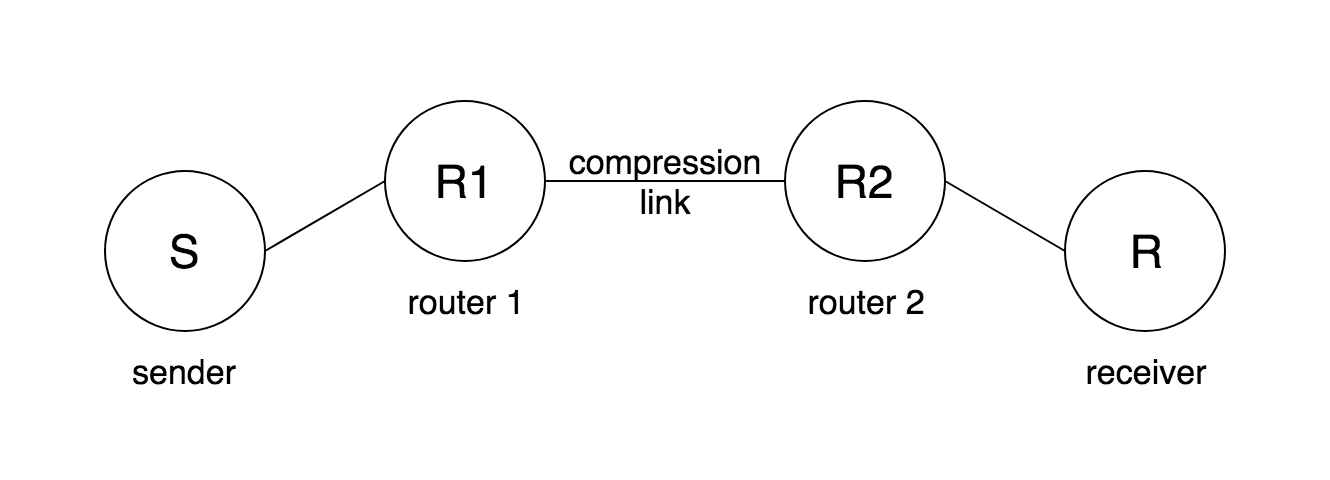
\includegraphics[width=\linewidth]{link_diagram.png}
  \caption{A 4-node topology with a compression link.}
  \label{link}
\end{figure}

\section{Submission Requirements and Deadlines}
You final submissions will be graded on design, implementation, code quality, coding style, and documentation quality. You will submit two documents: (1) Technical usage manual, and (2) final report. You should follow the \href{https://www.nsnam.org/develop/contributing-code/coding-style/}{ns-3 coding style}. While you are not required to submit a design document, you are strongly encouraged to maintain one in order to deliver your project successfully.

There will be an in-class project checkpoint on \textbf{February 14th}, where each group will discuss their project progress with the professor.

All code and the required usage manual, should be pushed to your repositories before \textbf{Thursday March 7, 11:59 PM}. Commits made after the due date will not be reviewed.

Keep in mind that at the end of the semester, you will present and demo your project \textbf{May 9th} in class, and submit a final report that is due \textbf{May 15th, 11:59PM}.

\end{document}